\documentclass[a4paper,12pt]{article}
\usepackage[utf8]{inputenc}
\usepackage[T1]{fontenc}
\usepackage{lmodern}
\usepackage[frenchb]{babel}
\usepackage{hyperref}
\usepackage{color}
\usepackage{graphicx}
\usepackage{shorttoc}
%\usepackage{layouts}
\parskip 6pt
%\hoffset -1.1cm
%\voffset -1.5cm
%\textheight 23.7cm
%\textwidth 15cm
%\headheight 0.8cm
%\headsep 1cm
%\topmargin 0in

\frenchbsetup{og=«,fg=»}

\begin{document}
\thispagestyle{empty}
\sffamily

\author{Rutkowski Juliette, 5a3DIJV \\ LABOLLE Victor, 5a3DIJV,\\Maître de mémoire : VIDAL Nicolas}
\title{{\Huge Mémoire de fin d'études / Graduation Memory }\\\bigskip{\Large Mods, game experience and game development~}\\\vspace*{3cm}{\large How to make a moddable game and why should I do that ? }}
\maketitle
~\vspace*{5cm}{
\includegraphics[keepaspectratio=true, height=2.5cm]{./ESGI-Logo.jpg} 5A 2014/2015 
\includegraphics[keepaspectratio=true, height=2.5cm]{./GES-Logo.jpg}}

\newpage ~\newpage
\shorttableofcontents{Summary}{1}
\newpage ~\newpage


\section{Introduction}

What if you could change something in your life ? What if you could add something crazy or magical in your world ? What if you could be someone else, with amazing abilities ?

Thanks to modding, this is possible.

Modding started with Doom, and became widely famous with Chex Quest, distributed as CD-rom in cereal boxes. Instead of a little toy, you get with your morning breakfast a 3D FPS non-violent. This promotion campaign increased the Chex sales by 295 percent. In fact, Chex Quest was a mod of Doom, designed to suit children and where you played an anthropomorphic piece of cereal.

Using the mods, Chex company removed the violent content (which was very controversial at the time) to create a content suitable for children that many parents were eager to buy. They greatly beneficed of this development and opened the way for a whole new gaming industry.

Nowadays mods rule their kingdom in the gaming industry, providing more and more content to games that are always more interesting. I can kill dragons in Skyrim AND fly AND stop time. Because I want to. I can survive in Minecraft AND play with pokémon-shaped animals AND use super powers. You can play a deadly Heavy armed with big gun in Team Fortress AND wear a fancy hat. Everything, almost everything is possible.


Being able to create a game which can appeal to every one of your players is a game maker's dream as well as a self extracting golden mine but, what are the factors that make a game appealing to modders ? how can I create a game that will continuously evolve over time ? and, well, why should I want to do that ?

In order to answer those questions and some others while we are at it, we will start with some definitions, then we will try to analyse some modded games we know about in order to see what modding added to player's experience, then we will see how modability is currently achieved. Then, we will think about why, as a game industry's actor, you should care about mods. And finally, we will see what you can do to make your game the most appealing to modders.


\subsection{Why this document ?}

Mr Labolle's word:
I've always loved to play with my games' data, create new things, alter others and test the limits of every single game I can lay hand on. But now I am going to work for the video game industry, I can't help but asking myself "how can I create games anyone can modify to fit his/her needs ?" and "what does it takes to create such game ?". I started those researches in order to find an answer to those two questions, hoping it would help me creating more flexible games in a first time and maybe helping other to create mod-friendly games for generations of modders.

Ms Rutkowski's word:
My first modding experience was in 2004 with Warcraft 3, when I first started to create maps on the Age of Empire map editor. At first I just wanted to create huge battle of hundreds of units battling in an improbable area, or artistic figures aligning units. Then I discovered Warcraft III and its battle.net with tons of awesome mods which were far more enjoyable than the original game.This was also my first meeting with online gaming and gaming community. These two concepts are highly related in my mind. I'm more of a consumer than a creator of modded content, and with that our work with Victor was highly profitable. We disagree on many points and that emulated our research, to prove each other our points' worth.

\subsection{What do you mean by "mod" ?}

The word Mod is to take here as a shorthand for "game modification". We might also use the words "modding" for the fact of modifying something in a game, "modder" for somebody who create mods and "moddable" for a game that possess the ability to be modified.

A mod is everything that alters the way the game is originally meant to be played. Said unmodified game is usually called "vanilla".

Mods can take many different forms, we usually classify them based on what is changed, we talk about graphical mod if the purpose is to make a part of the game look different, we talk about item mod if the purpose is to add or modify new items and we talk about core mod if the changes are concerning the game mechanics. We usually use the term "replacer" when the modification consists in change one asset for another and when a whole new game is created through the process, the mod is usually called "complete conversion".

As a result, mods can make the game much heavier than the "vanilla" version, and may require much more power from the computer. Depending of the skill of the modder, the mod is more or less optimized and can impact strongly on the performances of the game, or even badly interact with other mods.

\subsection{Different types of mods}

Mods can generally be classified in two categories :

\begin{itemize}
\item Graphical mods: Change the visual of the game. Add new textures, shapes, models and shading effect to a game. Can also modify the user interface. Those mods are less likely to impact on the balance but can impact performances.
\item Content mods: Add actual content to a game like quests, non playing character, items, weapons, class, events, spells, races... Modify deeply the game data and is likely to be unbalanced. This modding is often banned in online game because it can be resulting in cheating (all players must be equals).
\end{itemize}
For a quick illustration of what can a minor change do, see those two pictures, here is the same spot (riverwood in skyrim) with two different graphical mods :
The first one is meant to enhance realism, thus slowing the game down a bit (or a lot if you have a normal computer).\\~\\
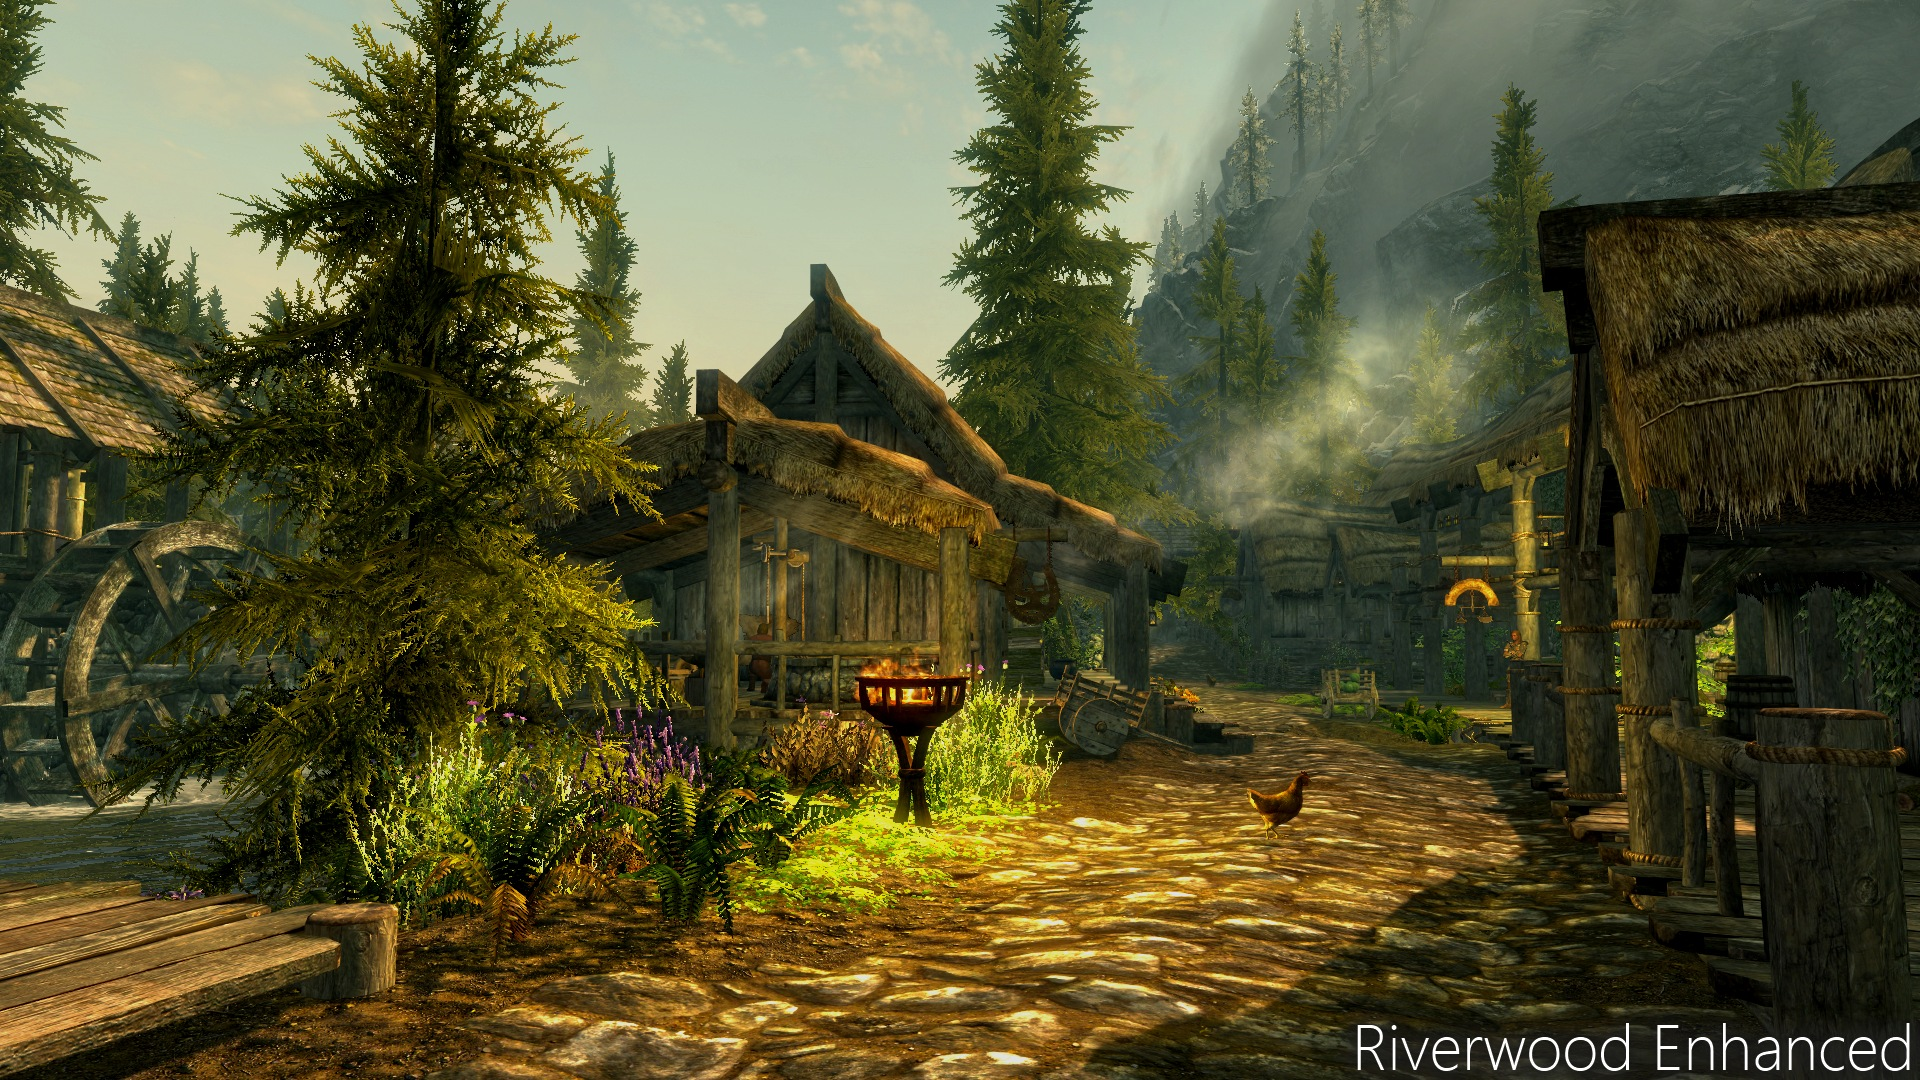
\includegraphics[keepaspectratio=true, width=13.7cm]{./riverwood-HD.jpg}

The second one is meant to improve performances by reducing the graphics, hence giving the game a whole different aspect.\\
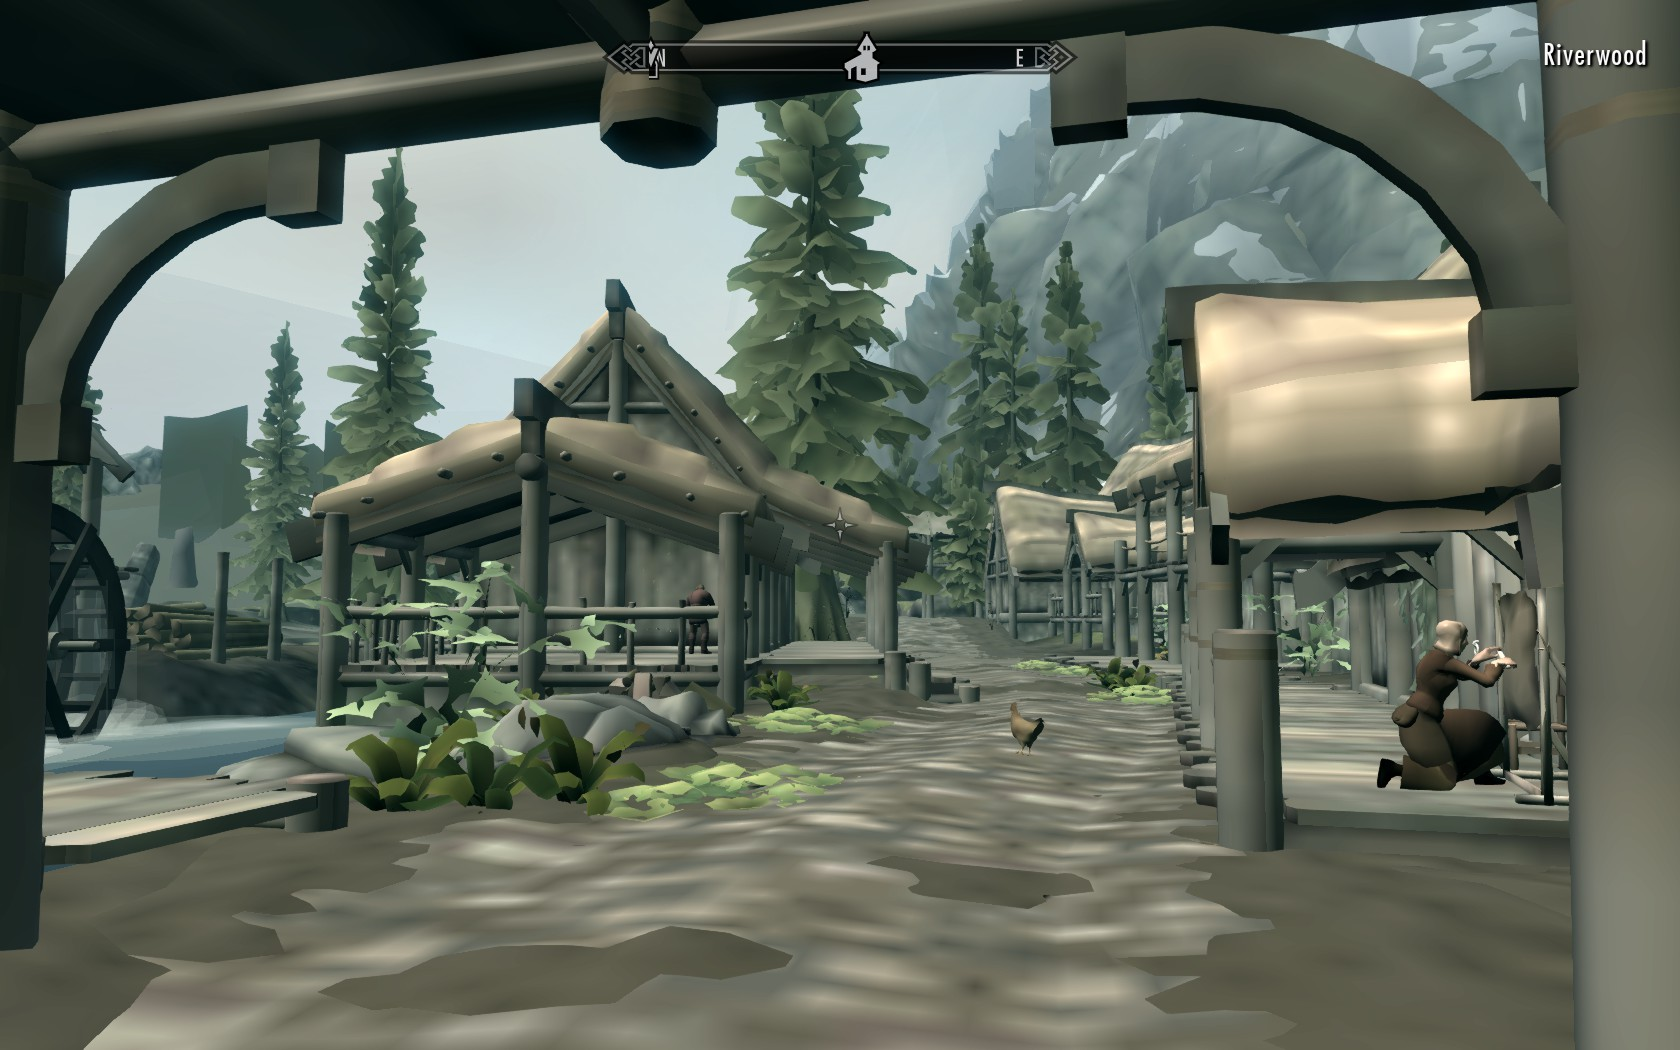
\includegraphics[keepaspectratio=true, width=13.7cm]{./riverwood-LD.jpg}

Some games use only graphical mods (mostly online games like World of Warcraft), or allow them only in local mode (you can't play online with an overpowered weapon that can kill every and each of your enemies). I can be very important for phobic person, who can't stand spiders for example. You can change the spider model by something less scaring so you can really enjoy the game.

Many games allows both mods (like Minecraft that is natively displayed in a low definition cube-like texture, and can be improved from 64x64 to 1024x1024). It's the case of most solo games (Mass Effect series, The Elder Scrolls series...)

When a franchise has an history of modding it can be very difficult to turn back and sell a "non moddable" sequel to your game.

\newpage
\section{Famous Examples}

Disclaimer : We do not pretend to present a full list of every single game which has been altered through the time but rather a list of games that we know have been altered and a little explanation on what it changed for the game and the player's experience.

\subsection{The ones who were intended to}

\subsubsection{The pioneers}

Doom and Quake saw their engine released, first under non commercial licence and then under GPL. Those engine were heavily used due to the fact that their creators were considered as really good and their flexibility.

ID software developed some games that posed as a standard for years to come. One of them was DOOM from which originated the "FPS" genre. If DOOM was not technically the first, ID Software were indeed the first to propose a "true" 3D environment with walls and items not placed on a 2D grid on the floor (the opponents were still 2D sprites though).

This was an achievement given the system capabilities back then and it is no surprise that whenever they decided to release DOOM engine's sources 4 years later, many people looked into it and tried to use it too.

The next highly popular game from ID Software was Quake which, this time did not render sprites but full 3D enemies. And, when its sources were released a few years later, the quake engine inspired many others to either fork the project either use it as engine.

The two engines were released roughly at the same period and were hugely used to make indie games or simply to develop faster. Those two allowed many ideas to take form and many games used those engine.

Many mods of those two games were in fact conversions in order to do whatever they wanted. Actually, publishing the sources of a game engine is somewhat different from what you might call modding because, at the instant the engine's developers published their engine as a tool to use, it was not using a game in a way the developers did not thought about but rather using a tool to create a game.

That's why we did not put them as games moded but rather as reminder that one day, people did an amazing thing, released it for free and this thing is still used almost 20 years after and by releasing those engines, ID Software allowed the video game to take a huge step forward.

from those two engines, a company made a game called Half-Life which would be modded to create a new game : counter strike. Years later, this company developed another famous engine called Source engine but we will develop later.

\subsubsection{The Elder Scrolls series}

This series and the third instalment of the Fallout franchise have been developed and published by Bethesda Softworks. They share an editor, improving it for each release.

The history of the Elder Scrolls' series modability starts in 2002 with The Elder Scrolls III : Morrowind which is the third instalment of the franchise. Upon install, you had the opportunity to install the now famous "The Elder Scrolls Construction Set" (usually called TESCS) which allowed you to, not only to change anything you want within the game but also create your own content and pack it so you could share it all around the world.

That simple possibility, given to the player to become not only actor but creator of his/her own story made his/her way in the mind of many players and led to the insane amount of mods this game has known since then and is still knowing.

What made it a good game and why is it, not only still played but also considered by many as better than its two sequels despite having clearly dated graphics, is subjective, but the fact is that the modding community around Morrowind is still active.

The Elder Scrolls IV : Oblivion was released on 2006 and, due to its heavy requirements for its time, many players kept playing and modding for morrowind but, lured by the shiny graphics and helped by the machines increasing capabilities, this game ends up seeing a fair amount of mods and players.

This time, the editor was distributed via Bethesda Softworks' website and the updated graphics and mechanics induced a significant increase in the editor complexity which might have prevented some morrowind modders from doing so with this new game.

The engine has been reused for Fallout 3, refined further for fallout New Vegas and so was the editor. Those two games are not part of the series but they share the engine, the editor, the developers and even some core assets so it's worth mentioning.


The Elder Scrolls V : Skyrim was released the 11/11/11. Due to an extensive advertising campaign, the fans were expecting it and, if the requirements were still high, they were nothing like the previous instalment was for its time (oddly, skyrim needed slightly less power to run in medium high than oblivion in very high).

Bethesda assured that their engine was brand new and, be it a simple (extreme) optimization of the old gamebryo or an actual new, it does not really mattered, the changes had few impact on the game's folder organization or the modding system.

Fun fact is that the first mods were made only a few days after the game's release, there were mainly ergonomic mods (the one I use on daily basis was first released after 2 days. It was simply meant to adapt the menus to a pc).

Three month later, when Bethesda finally released the editor, it has, again, changed a lot. Bethesda however released with it video tutorials and a wiki in order to explain how to use the editor.modders, leaving, again, time to develop DLCs and still having people to buy them.

%\includegraphics[keepaspectratio=true, width=15cm]{./images/VG3Cs.jpg}

\subsubsection{World of Warcraft}

World of Warcraft was announced by Blizzard in September 2001, publicly released in November 2004 In USA, New Zealand and Australia, and in Korea and Europe in 2005. First, players were allowed to register some macros, then full "add-ons" were developed and spread in and by the community. These add ons were meant to only be "visuals". World of Warcraft being a Massively Multiplayer Online Game, each player had to be equal in term of content, stuff, non playing character...
Many of these add ons help the player to manage his/her interface, to give him more information about quests, bosses, rare mobs, way to improve reputation for a certain faction... One of them, GearScore, gave a "level" to each item depending of its stats, and this add-on became preponderant to rank a character, even leading to excluding some players, their stuff just were not good enough to take part in raid or dungeon.

In a result, when Blizzard released the biggest update for World of Warcraft, Cataclysm, in December 2010, they included to their new "vanilla" version a lot of the most used add ons. For example, the item level (ilvl)  (used by the add on GearScore) was used as part of the gameplay. Each player was required a minimum of mean ilvl in his/her stuff to apply in the dungeon

If these stories can be analysed, we can see that encouraging mods in the first place allowed morrowind to be played for a longer time thus giving time to develop two DLCs and still have people to buy them. Advertising and providing support to modders were great ways to attract new players and or raid search. It guaranteed the raid leader player with enough stuff to not be a burden, and hopefully a minimum of knowledge of the strategy.

This example shows that keeping a careful eye on mods created and loved by the community is a safe way to know how to improve your media. If most of your players want a specific interface upgrade, it can be a way to produce a better game. Also, a player who dedicate enough of his/her time to conceive and produce a mod is more likely to buy your next game or DLC/extension.

\subsubsection{Warcraft III}

Warcraft III Reign of Chaos, and then Frozen Throne is a real time strategy game released by Blizzard in July 2002. Even with the vanilla version, a map editor was released, allowing player to create their own maps, with factions, events, grounds, forest and shops entirely editable. These maps were playable in solo mode or even online with strangers. A lot of maps were created and some mods became famous and were transposed in other games when possible.
\begin{itemize}
\item Tower Defense : Waves of enemy mobs spawns from one or more points and follow a determined path. Each player can build tower to defend the path and kill the monster before they reach the end point. Depending on the version the player could even build his/her towers in shape of a labyrinth to lengthen the path of the mobs. One "official" Tower Defense map (Defense of the Crystal Tower) was released with Frozen Throne in 2003
\item Hero Defense : Lookalike of Tower Defense. In this mod the player control a single hero, based on hero and units from the vanilla version, with stronger and more diverse abilities. This mod is really focused on team play. A variant is Enfo, with two teams of 6, where players can use spell to annoy and handicap the enemy team. The remaining team was victorious.
\item Buy and Sell : 4 Players are sellers and try to get the better profit possible, the other players compete as buyers, trying to buy the more unit from the sellers to destroy their opponents. The buyers cannot buy any unit without the sellers .
\item Line Wars : Two teams of opponent players compete in a small symmetrical map to destroy the enemy base with the help of uncontrollable minions. Players can spend the gold earned on kills by improving their base and minions or upgrading their own stats.
\item Defense of the Ancients (Dota) : more codified and complex version of LIne Wars. Two team of five players battle in a large map with three lanes (path from one base to another) and
a "jungle" (wild forest populated with neutral monsters) wrapping the central lane. Both bases are represented by "Ancient" (animated tree of the elven faction of Warcraft).
\end{itemize}

The DotA mod was the most famous of all and was played by more than 10 millions of players. Later this mod inspired a new type of game : MOBA (Massively Online Battle Arena). Some games were created, inspired by the DotA mod : Dota2 (produced by Valve), Smite (Hi-Rez Studios), Heroes of Newerth (S2 Games), and most of all League of Legends (Riot Games).

As an example,  League of legends, in the beginning of 2014, recorded more than 67 millions of monthly players and 10 millions daily players. These games participated in the soaring of the electronic sport (e-sport). Big societies like Coca Cola, Samsung, BenQ, Asus, Razer, SKT Telecom invest a lot of money in e-sport teams and professional players, people win their life playing games, and the cash prizes has never been higher (more than 2 millions dollars).

And all that started with a mod designed by two young gamers in 2002.

\subsubsection{Minecraft}

Minecraft was an independent video game, type "sandbox", firstly developed by Swedish Markus Persson (alias notch), then by Mojang studio. The world is realistic but cubic, everything having a cube-shaped design. It was originally design for Web browsers, and after was available on PC, Mac and Linux OS. It's also available on Android and iOS devices, and was converted for XBox 360 in 2012, and PS4 in 2014.
Mojang studio and Minecraft was  bought by Microsoft in 2014 for 2 billions Euro.
Minecraft was sold in more than 54 millions of exemplars in June 2014.

The game principle is very simple at first. The player could move around in the world, gather wood from trees, dirt and stone from the ground, build some tools and try to survive in an hostile world. At night aggressive creatures like Skeletons or Zombies appeared around the player trying to kill him.
Through time and updates, two others worlds were created : the Neither and the Ender, were different creatures appeared, new items and above all the Redstone. This particular supply allowed to create logical system, using lever, buttons or pistons, to open doors, create traps, kill creatures...

In Minecraft, almost everything is moddable. The most known are Texture Pack, which change the original 32x32 texture by much better one, up to 1024x1024. They are the easiest to implements and use as a basic player. You just have to drop a folder or a zipped file in a specific folder of your computer and then chose it in your game. This way you can manage many textures depending of what you want to experiments.

For example, some texture packs are dark, detailed, for more immersion and role play sensation. Other are smooth, with nice colors for more relaxing and more recognised blocs.

Another way of modding Minecraft is to add game objects, passive and hostile creatures (Pokemon, dragons, Zebras) or even game mechanics (Survival Zombies mode where the spawning of mobs is increase by night). It is very easy to implements and the possibilities are quite infinite. Relying of the simple design (cube-shaped objects) you can include tons of models without issue.

\subsubsection{Valve, Steam \& Co}

Valve Corporation (formerly Valve Software, commonly referred to as Valve) is an American video game development and digital distribution company, founded in 1996. In 2003 they created Steam, a internet-based digital distribution, digital rights management (DRM), multiplayer, and social networking platform. On February 2015, 4500 games were published on Steam, with 125 million actives users and it is estimated that 75\% of games bought online are downloaded on Steam. The Humble Bundle Series help with this popularity by "offering" four to ten games per month for a very modest fee (1\$ to 15\$)

With the release of Dota2; Steam and Valve rushed for the first place of game platform. This famous esport game brought any players, the strongest communities being in Russian, China and United States.

The steam team has been trying to ease modding and user installation. For most of the steam games, mods are added to the game by browing the workshop and clicking the “subscribe” button on a mod which is automatically add to your game folder and menu.

Of course not all games allow mods and workshop but a lot of them does and steam encourage it, as we could see it with their initiative to allow "paid mods" which recieved mixed feedback.

\subsubsection{The Half-Life series}

Half-Life is an FPS (first player shooter) developed by Valve Corporation and published by Sierra the 19th of November 1998 (available on Steam since 2003). It was first designed for Windows OS and since 2013 for Mac and Linux OS. The game was very popular and many independent developers created even more famous mods of the game. Some even became stand alone games.

We talk about the Quake engine in the beginning of this section and the first half life engine, GoldSrc, is based on a heavily modified version of this engine. This game will know quite a success to the point to see a complete conversion of it becoming one of the most played game in classrooms.

This mod, Counter Strike is the first of a long series of FPS, and was published and sold with the agreement of Half-Life authors. It was based on Half-Life game engine, with two teams battling, terrorists and anti-terrorists.

Basically, the game was not designed to be moddable and first mods were kind of "hacks" of the game, illegal. But when Valve realised the hype around these games, they decided to encourage and promote the mods and released a free SDK to help the players design new contents.

Many official and non-officials games were and are released since Half-Life original release, keeping track of them is rather difficult and the fact that we both are not actually interested in the FPS genre don't really help.

The Source Engine has been developed by Valve after that and was first used for counter strike : source and then for the most known half life 2 which has known many mods and improvements, as we can see in the portal game, also based on source engine, where the player can literally connect two space points into one continuous which is quite interesting from a technical point of view.

Once again, the mods done with the half life series were more aiming to create a new game rather than modifying the existing one like you can see with the other games we presented here. Maybe this can be explained by the fact that as it was possible to create something new from scratch, people could not resist to do so instead of just improving the base game.

As the newly created game still needs the base game to run, this was not a bad move from valve because they end up creating a game engine with a way to still get money out of this.


\subsubsection{ARK:Survival Evolved}

ARK : Survival Evolved is developed by Wild Cart Studios, as their first game. The game takes place in a strange island filled with prehistoric-inspired animals, like dinosaurs, ancestral monkeys and aquatic mammals. It is currently in early access, starting from June 2015. Of course at first, no modding was included. But the game was immensely praised for his active dev team, close to their community and fast to fix bugs. Adding features was also a weekly engagement by the team that was very appreciated by players.

ARK is based on Unreal Engine 4 and therefore has a special way to give access to mods. You can download the ARK Dev Kit directly from the Unreal Engine 4 launcher. Modding for ARK use the Unreal Editor so users familiar with the engine can learn fast how to mod and share their work. A negative point is that the dev kit include all the content of the game and need a huge memory space (more than 40 Giga).

In a bit less than 3 months, 343 items have been added to the Steam Workshop, making it a large success in term of popularity.

WildCard Studios also organise a huge mod contest starting in November, with cash prize of 15 000\$ for the winner plus a alienware computer and a graphic card. This encourage a lot mod authors, giving more and more reasons to create content.
With its state of early access, the game only include one map (large enough for any new player to get lost, given their position does not appear on it). The contest focus on two categories, new maps and new game mods. And the workshop is now filled with new items, new game mods (more aggressive dinosaurs ? nocturnal attacks ? All you want you can get).

This is a very good example of how modern games can implement mods in a simple way to be used, and also give a fancy example on how using a native game engine can ease the modding process.

\subsection{The ones which were not (but ends up being anyway)}

This section lists some games that were not meant to be modified, yet have a community trying to mod it and that I have personally tried to mod. There are obviously many more games that would fit in this but we would rather talk about something we know about.

\subsubsection{The Fable Series}
Fable is a game made by Lionhead studio and published in 2004. Its director was the now famous Peter Molyneux, also known (and sometimes hated) for Curiosity - what's inside the cube ? and generally speaking for overselling even bad ideas.

Although this game had a classic scenario and a really Manichean view and morality system, the graphical choices were good and if the 3D is now clearly dated, the light and the artistic style make it still relevant.

Whenever a game shows potential, people try to see what they can do with it. Sometimes, a guy crazier than the others create a tool and release it. That is what happened for the first Fable game, a guy released a tool called chocolate box which allowed to modify the game data. This editor was quite impressive for something done by an amateur.

The data was stored in a big compressed file, for any modification, you had to extract them. It's also a requirement to use chocolate box. Modding is relatively easy as long as you don't want to do anything complicated like adding quests or building a city.

Although an editor has been released, the community was not that developed and, if there were mods done, it is nothing compared to many others moddable games, mainly because installing is not easy, mainly because having two mods at the same time implies merging text files, which is uneasy.

The second episode was console only so, if you are looking for mods, there is no hope so nothing to say about it.

The third episode was meant to be played online with a friend or a complete stranger. As such, Lionhead tried to prevent cheating to make it fair even though it was a co-op against environment. It was made so it would be complicated to change things, the save is encrypted, the data too and, anyway, there are checksums that ensure nobody gets interested in touching their game. As a result, there were not any tool made and, to be honest, the critic reception of this episode was not exactly good so that might explain why there were not many attempts to crack the security in order to mod this game.

As for public reception, the first episode is considered as good but the third is rarely mentioned. The moddability of these games do not have anything to do with it but it could have greatly helped since what is commonly reproached to the third episode is that it is too short.

\subsubsection{The Sims series}

The Sims series have been around for a long time now, those games has been modded since the first opus and although many different editors have been created by modders, the process is still fairly painful. However, due to the huge potential of modding for a sandbox game and the high number of fans, the modding community around the series have always been active. As a matter of fact, the sims are one of the games with the most of graphical content available on the Internet.

Disclaimer : all what we say here is verified for the sims 2, we never had the occasion to try modding for the first game.

This one is rather interesting because the moddability was intended as a way to make profits by selling additional content as do Maxis since 2000. Each and every iteration of the game saw plenty of add-ons and expansions, not mentioning items sold separately. Maxis never gave players the tools to create and share content however, they did something clever from their point of view : they made game modifications really easy to install, just double click on it actually. This way, the players were customers for (official) mods, everybody was able to get them so, like I stated before, the very concept of the game calls for adding custom content.

If modding taught us something, it's that no game company can be as creative nor as productive than its player community so, if your game is interesting enough, there will always be somebody to find a way to make some modifications. That's what happened for the sims, as mod distribution was easy, all what left was to make tools, which was done pretty quickly because the sims' fanbase is fairly huge.

Until the third instalment however, the modders were not exactly helped by the developers and installing a mod was more or less complicated depending on what you wanted to be modified. But since, they simplified the way to install mods, without changing too much how they are made which helped modders to adapt.

The way this series is treating mods, as custom content, is interesting. They actually make a little difference between the paid additional content they sell on the online shop and the content made by fans. The only difference being the little icon stating "this is custom" or "this is from the shop". Some custom content is actually sold but that is somehow illegal.

\subsubsection{The Mass Effect series}

This series have known a great success and the games are great but modding for them is a real pain. Like many game companies, they made their game so data are difficult to reach. Be it intentional or not, it does not matter, the fact is there is an editor, again developed by a fan, which allows to modify some values but it is tedious. There is a community of modders, but they are few because of the difficulty of modifying the game and the limited amount of possibilities.

The Mass Effect Series were developed by BioWare and released between 2007 and 2012. A fourth opus is announced for 2016. The story takes place in a sci-fi universe with many different extraterrestrial species and planets. The first game was quite a success but was never meant to be moddable. Essential data was hidden deep in the code, hard to modify except for "I like danger" modders. It makes mods hard to create, hard to share, hard to install. Nevertheless, the modding community is still strong supporting the game. From shared saves to updated HD textures for the first game to catch up with the advance in technology, mod authors still find a way to improve their gaming experience.

Quite a few of these mods are based on user interface and controls. For example, there is a mod only dedicated to using the xbox controller with Mass Effect 1. Many players like to use a console controller on their PC games. It can sounds strange but some players are really better with this controller and enjoy the game most. But the Mass Effect 1 game for PC didn't support the other platforms' controllers. The user interface is also slow and not very friendly if you compare it to the third opus. The fresh paint on the game maintain the players' focus and interest.

But it's very clear that the Mass Effect Series weren't designed for mods and are very mod-phobic. Creating a mod includes extracting files, modifying them,  repacking them and pray that everything rules at its finest. Some simple mods about textures take 20 steps to install for the user. Data is saved as pairs of key and values, not easy to understand and modify. The more complex mods modify all part of the game, removing some dialogue lines or rearranging the way the scene are ordered to create a really different story. Mass Effect 3 has been very criticised over its ending and mods can help you have the perfect ending that you desire, save a character, or delete one that you don't like out of the game. Mod author achieve so by mostly modifying dialogue lines and conversation trees.

\newpage
\section{How is modability achieved ?}

Bethesda's way of doing it (The elder scrolls, fallout 3 / NV) : From a technical point of view, the ability to modify the game relies on the fact that all data required by the game are stored in a folder. It contains archives which are the game's original data. If you want to modify something, you just need to extract it, modify it and leave it here. By default, the game will first take the files in the folder rather than those in the archive. If you want to change game data other than assets, you can use the editor released for the game you are using, thus creating a .esp file and activate it in the game launcher.

Maxis' old way (the sims 1 and 2) : they don't exactly encouraged it but they certainly did nothing to stop it. As tedious as it can be, the game data (and there is lot of them) are all stored in one single archive file. If you want to modify some core aspects of the game (such as item cost, time needed to perform specific action or the impact of a skill), you have to extract the corresponding xml file and alter the corresponding field. This may be tedious but it is rather simple. Oddly enough, adding models to the game is not as easy but nothing can stop people from adding new stuff to a sandbox game...

Maxis' current way (the sims 3 and 4) : now, mods have their directory, you just drop your files into it, activate them in the launcher and you are good to go. There is also an even simpler method : if your mod is a .package, you can simply extract it with the game launcher and that's it. This can be an example of how to do it right for the install part. That said, modding for it is still a pain.

Bioware way of not doing it (KoTOR, mass effect, dragon age): game data are stored in a .bin file, as key - value pairs. It might be far easier for the game itself but it's definitely not modder-friendly. The only way of modding is to alter said .bin file so, you can only have one mod at the time or merge it yourself.

Lionhead way of not doing it (fable) : very similar to the previous one, the data are stored in a huge file and extracted. To modify something in the first episode, you had to use the fan-made editor. In the third episode, the save and the data were protected by encryption and not any editor was released.

Mojang's ways (minecraft) : there is a mod toolkit to help modding, wikis to help installing them. The game started as a community and, even if it is not a free game, the community is still really strong.

WildCart way of dodging it : they are releasing the devkit as a module for Unreal engine, that way, the installation is easy (but huge) and give the modder a great freedom. Installing a mod is done via steam, by clicking the "subscribe" button, steam takes care of the rest, which can be considered as easy installation. Although they are using tools to achieve it, their choices made everybody's life simpler.

\newpage
\section{Overall benefits}

Modding makes a game go beyond its vanilla version, and give it some replay value for the player who liked its first run. Many players would not be interested in mods unless they already got a strong interest in the game and want to know/have more. Some others however, would love to play your game but can't because of some random reason like arachnophobia (Why did it have to be Spiders ?), realism (so, I am a gun ? and where are my foot anyway ?) or because one item is missing (lightsabers, lightsabers everywhere) and then, a mod appeared, doing just that, making the game playable from this user's point of view.

For example, The Elder Scrolls series has as a vanilla version a huge world and amount of quest and npc. Most players will not get interested in mods unless they already feel they complete most of the game by themselves. Modders are often players a bit frustrated by a part of the game ("why doesn't this spell exist ? I should invent it !") and try to improve their own game experience.

\subsection{The editor's point of view}

As an editor, allowing mods can be of a great benefit. First of all, it is a great way of developing a community around a franchise which means more people talking about your game and more people who might buy any sequel. Then, as long as the community is alive, it will draw more people to buy your game, either because some new awesome mod caught their interest or just because they only hear about your game now (sales can help too)

The editor cannot presume of what the player will like, dislike, and what will make the player keep on playing. In extension, it is hard to know if a player will create mods or no. Essentially, a person who already has created original content on an other game will be more likely to create on your game.

In consequences, if you provide the most complete experience while giving the possibility and tools to improve the world and go further and deeper in the world, you will gain more loyal players that will keep on working on the game years after your release (eg. Morrowind from the Elder Scrolls series, still has an huge fanbase community that keep alive the spirit of the game. In extension the mod Skywind will use the graphic engine of Skyrim (TESV) to create a clone of Morrowind (TESIII)).

Economically-wise, if your game is modded, it will be played longer than average game. This means you get more time to make DLCs. However, you have to be careful when releasing such DLC because if your modding community is good at making new complex and rich content, you will have to show them why YOU are the ones who create games for a living.

It also mean that you should create a support or tools to gather your community (like forums or ticket system)  and manage it efficiently.


\subsection{The developping team's point of view}

As a developer, thinking of a "moddable game" is a strong force in the development process. You have to think, analyse and prepare the field for any modified content. It can be a burden, especially if it is their first big project. It is very important to plan the process, specify which should be modified and which should not, ideally, everything should be modified, configurable or tweakable but we all know that video games are all about performances so you have to find the balance, which might be an interesting challenge.

As a 2D/3D artist, you have to make sure you are using the right file format and, when creating assets for level designers, you might want to make them all on the same size. Bethesda explained how they do that in a tutorial about level design, explaining that every single asset for dungeon crafting is roughly of (a multiple of) the size of a cube, guaranteeing that every piece connects seamlessly , thus, facilitating dungeon crafting.

As a level/quest designer, you will still have to think about your levels beforehand but a level editor can make this so much easier, allowing you to see what you are doing in real time and, the more powerful your developper made the tool, the more efficient you will be. So, be nice with your developers, report bugs and try to figure out their origin, you will see, they like this.

Now that we discussed about the benefits, we have to be fair and say something about the drawbacks. Developing a good modding / editing tool takes time, patience and a lot of debugging, which basically translate into : more expensive game and more delayed release.

So, why would anyone want to do that ? well, if you are planning on releasing one game and stop, yes, it is useless. However, if it is your job, chances are that the tool you used on the first game will be refined on the next one and so on, leading to, not only a tool which is slowly getting closer to perfection, but also, assuming you release the new tool with every new game, you will familiarize your modder base to your tools, thus making modding easier for them for every new game.

To summarize, by refining your modding tools on each game, you create a base of modders that progressively learned to use your tools and that you can eventually end up hiring without having trouble to form.

However, If you decide to release fast a prototype and get over with it, you might want to forget about the whole editor thing because it is massively time and money consuming. But, you might as well want to try a game engine like unity or unreal.

\subsection{The player's point of view}

As a player, each person looks for a different game experience. Some players will play only vanilla version of each game they try or buy. They are just not interested in creating content from their own imagination.

Some players will use mods, but only as consumers. They will install mods, try them, make critics but never create by themselves. Even if they don't contribute materially to the modding community, they keep it alive and have their interest renewed from time to time by new mods. These players are often emotionally linked to the game, share memories about it and are often loyal to the franchise. They also feel like being part of a community ("those who went beyond the original game"). It is always rewarding as a player to feel like you are part of the "elite" or "the few ones".

for those players, the benefits are obvious, they can pick the mods they want from the community, adding, removing, modifying what they want, to the point to fine tuning they experience in order to get the optimal experience. They are usually more prone to buy good quality DLC but might be quite picky if said DLC is of lesser importance like, say, a horse armour...

Finally, a few players will create content on your game if they can. It is kind of an "engineer" state of mind when you "have" to understand how the game works. Theses players, when they start a game, quickly go to the step "Is this game moddable ?" and then start trying things, conceiving small add ons and enjoy the game more this way. They feel like they create their own experience of game, personalised, that really suits them.

For them, the benefits are even bigger because they can play the game, then play with the game, then push it to its limits then create and then play with they creations. It is a whole new world to explore, a feeling of power... Often only ruined by the engine limitations.

There is conflict and debate among the gaming community about whereas you should play the vanilla version prior to use any add on or mods, shall they be visual or content. Some players argue than you should honour the developers' work by playing the original version, to see really what the game actually is. It allows to fully enjoy the new content by comparing with the vanilla version.
In an other hand, players prefer to play directly with mods to have a stronger first game experience, with less bugs,

%\section{Drawbacks }

%\subsection{The editor's point of view}

%\subsection{The developer's point of view}

\newpage
\subsection{What are the gamers expecting ?}

\subsubsection{Data and deductions}
We conducted an online study on 530 persons that identify themselves as "gamers" (they played video games quite regularly as an hobby). Most of them were teenagers or young adults between 15 and 21 (respectively 33.6\% and 38.1\%) and a quarter (25.2\%) were adults older than 21.Half of them played more than fifteen hours a week (53.7\%) and a bit less played between five and fifteen hours a week. We can call them regular players.
We asked them if they used mods in games and why. Here are the results : \\
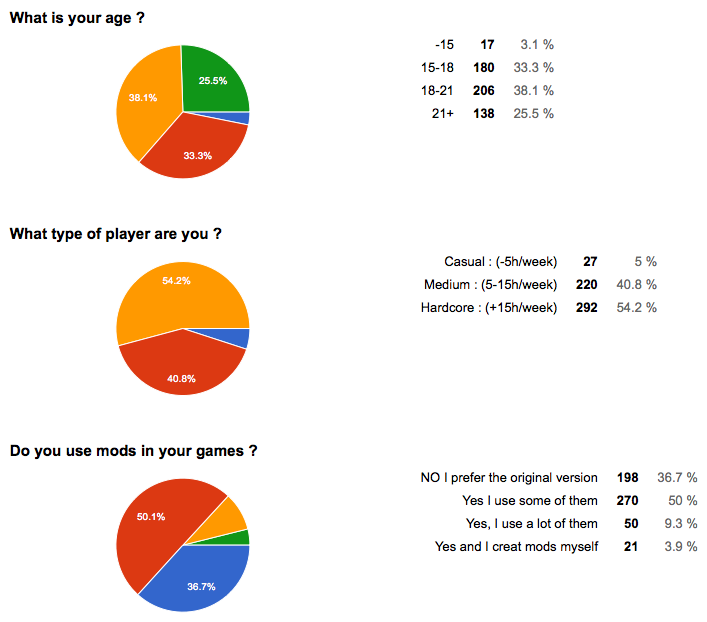
\includegraphics[keepaspectratio=true, width=13.7cm]{./uberCharts1.png}\\
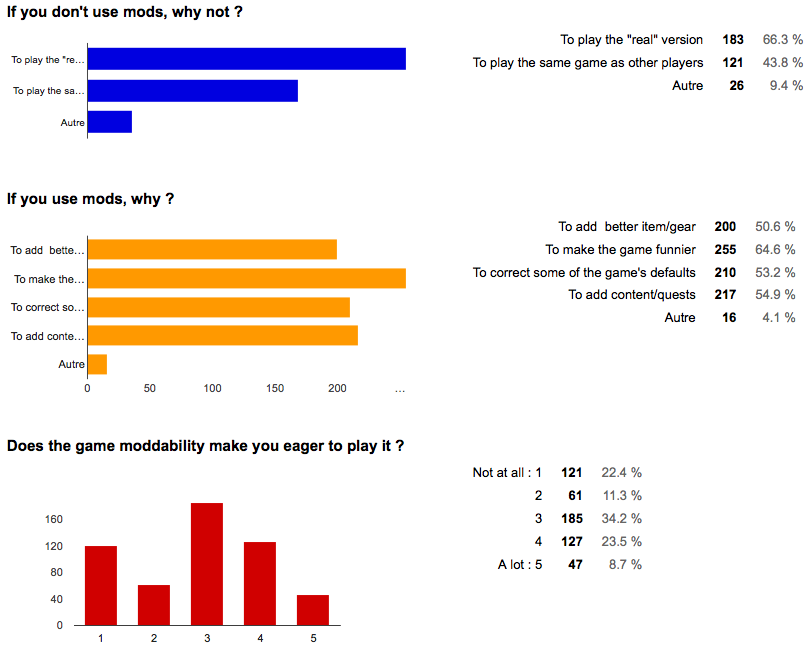
\includegraphics[keepaspectratio=true, width=13.7cm]{./uberCharts2.png}\\
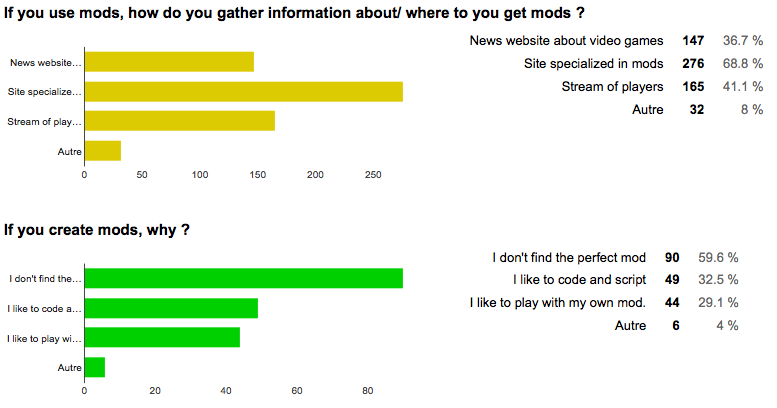
\includegraphics[keepaspectratio=true, width=13.7cm]{./uberCharts3.png}\\

We see clearly that a good third don't use mods at all (36.4\%). Most of them want to play the original version, the "vanilla one" as we called it. For some of them it's also to play "the same game as other players", whereas it's an online multiplayer one, or to share the same experience and be able to rely on shared feelings and sensations.

Playing a game with and without mods is a very different things and it can repel people from using mods.

Some players also stated that they didn't use mods because they didn't know how to do so, they were afraid of technical issues, or their computer wasn't powerful enough to run the game with one or multiples mods.

You must also be careful that mods don't interfere with the good running of your game and don't slow it down too much.

For thoses who use mods, they admit they use only a few of them (less than 10 per game).The majority want to improve their game experience by adding content to the game. Concretely it can be new weapons, new clothes, new body models or even new buildings.In an other dimension, it can also be new quests, new regions, new characters, new game mechanics created from the original one. As an example, Minecraft modder's create whole "adventure maps" where game mechanics

A huge argument for mods is also to make the game funnier. Because yes, it's awesome to play a dragon killer, but it's even more awesome if you can do it with a rabbit with a backpack as a companion and a boar in place of your horse. Fighting against skeletons and zombies is nice in minecraft, but it's even nicer if you can catch pokemons along the way.

Half of the users specify that mods were used to correct some of the game's defaults.  This reveals a lot about the players' frustration and how they manage to control and override it.
Unlike a book or a movie that is written from A to Z without any possibility of change, moddable games can be rectified when bugs are too obvious or difficult to handle. Answers really want to point that modders shouldn't do the work of developers (pointing out especially  Skyrim that needed a huge amount of patching and modding to be playable.

More than simple mod users, 4\% of our answer base create mods themselves. When we asked them why, More than a half declare they don't find the "perfect mod", meaning they didn't find any mod than match their desires. The databases of mods keep growing thanks to modders frustration and will for perfection. Of course not all modders publish their mods online for other players to use, but those who do so on platform like Nexus or wiwiland encourage player to challenge the game in a totally new way. Players massively gather informations about new and popular mods in specialized sites like nexusmods, wiwiland, mod section on official site, steam workshop related to the game. A third of the answers also state that they get inspired by streamers playing special maps or mods. The efficiency of streaming is not a be discussed any more but it can be increased by adding mods. You can make a gamer play your game again if s/he spots a nice mod. Streamers often promote games and encourage viewers to play the game with a new point of view or a new dynamic.

We also asked "if the game is moddable, will it make you eager to play it ?". Two third of the answer were positive, having the possibility of mods has a positive influence on perception by players.

\subsubsection{Study conclusion}

We could notice some important points from the study :

First of all, people like mods and want to use them. They want to experience and share their experiences. Mods are a social dimension of games and promote the game and its players. They emulate the community and encourage creativity. Through sites, forums, gits, modders and users connect and encourage each other.

Then, mods are meant to expand the game, not correct it. Having the possibility of mods doesn't prevent the developers to finish their game properly. Mods don't discharge the studio of all of their responsibilities. Players expect a clean and useful product to play and work with. Modders above all need a sane game to start with.

Finally, players are reluctant to use or create mods because of technical issues. Making sure you got a clear and simple way to use mods (like a "Mods" directory)

\newpage
\subsection{Mods and business}

At first mods were all free. It was just about adding custom content to a game. But nowadays, different business models are used by editors.

Maxis, for example, sell some item packs in game for The Sims series. They also have a "gallery" where creators can publish and share their new clothes, buildings, rooms or hair style. Mods by community are free of charges while mods by Maxis cost a fee.

In April 2015, Valve and Bethesda released "paid mods" on steam, meaning than creators could sell their mods instead of giving them for free. It was meant to give creators the opportunity to live of their work full time if they got success. But the community reaction was so violent Steam cancelled the operation 4 days later. The main argument was about the repartition of the price between modder and editor. The modder received 25\% of the price and the rest was shared between Bethesda and Valve. The community reacted violently to this announcement stating this was a betrayal by Bethesda.
As Steam stated, paid mods can work and do work in other games, but the Skyrim community was old and well installed in the steam workshop and not willing to adapt this change. It may not be so easy to bring paid mods in your business model if you community is used to a different pattern and the modder's share of the fees must be enough to justify it.

Steam is a very good example on how mods can easily be integrated to the original game. In most of games on Steam, you only have to click a "subscribe" button on the content you want to add to your game and it's done.

Done, but not all the time...

In some games, mostly those in early access or/and with custom values to .ini files, the modder may provide a step by step installation guide. This applies mostly for deep modifications like "max player level", "max health points", that can't be modified through an editor.

If you intent on releasing your work on Steam, as it's massively done these days due to Steam popularity, workshop and mos are a huge part of the community grows. As example, ARK Survival is still in September 2015 in early access mode, and due to this particular state the workshop wasn't open before July 2015. Only two month after, more than 340 mods are released on Steam workshop,. From being able to grow dinos eggs to a totally different map or new ways to build, creators learn to build new content from the few tools offered by the ARK developers. Being an early access, it only have one map available at the moment and people were starting to struggle and complain about the lack of novelty in the game, despite the new dinosaurs and game items added regularly.
The workshop added new energy and some fresh air in a game that still need some months of development.

Deciding to made paid mods available is a strong and important decision. Even if the modders won't produce content as valuable as your own DLC (at least you wish), it may restrain players to buy the said DLC, because they prefer saving money for funnier mods, closer to the user in fact. They also may prefer to support modder instead of you, the editor. If you are still willing to allow paid mods, be careful about the mount you share with the modder.

\newpage
\section{Requirements}

In this section, we will think about what does making a moddable game implies. Those rules are obviously not mandatory and many moddable games don't follow them all but, from a modder's point of view, they are most welcome. And you will see that you have many reasons to please your modders.

\subsection{General advices}
Making a moddable game can follow the same rules than a group project : the file organization must be clear, documentation must be precise and, if possible, easy to access.

The easiest to understand your organization is, the more modders you get. The more modders you get, the more content they create. The more content your game get, the more appealing it gets to new players. Easier said than done but if the job is well done, your game may still be selling after 10 years like Morrowind does (just look for it on Steam).

You might also want to try out a ready to use game engine like unity or unreal, their file organization will force you to organize your files in a defined way, making modders that are familiar with those engines to more easily understand your organization.

\subsection{Architecture}
The last paragraph stated "the file organization must be clear" which, ironically, is as unclear as it can be. So, we will think about how files should / might / can be organized in order to avoid trouble in the conception phase in a first time and make your game more appealing to mod in a second time. But, for starters, let's discuss some little details about general coding.
As many games are not done from scratch nowadays, we will not spend days discussing game engine and how they should be done... That said, for the three remaining ones, it is important to keep in mind some little things :
\begin{itemize}
\item Modding is experimenting : never say "there will never be a negative / excessive value". You must expect your players to try things. Negative gravity value or five billions gold are frequent modder's try so, either shield your inputs and test for overflows or, better, use the most generic functions you can.
\item Modding is forgetting things : always think about a default file in case you can not find the one requested. A silent sound, a default mesh, even a doNothing script... Your level designer will be happy to see your defaultTrollFace.obj instead of crashing back to his/her desktop without any explanation.
\item Modding is 90 percent testing, if something goes wrong, say it, preferably in game in a pop-up window explaining the error clearly with three buttons : "continue", "crash" and "continue for all". You might also put these in a log but with parsimony, those files can become huge...
\item Modding is often wanting to do something new / unexpected. So, if you can think your code to be able to include add-ons, you might create the ultimate moddable engine.
\item Modding should not be about learning new custom / obscure languages for every new game. When you have to script things, think about already existing languages rather than creating your own. Javascript or python can be an excellent choice.
\end{itemize}
Now that I defined what modding is, let's talk about the elephant in the room...

You can have a perfectly moddable game and a huge community of modders if every mod is a pain to install, only a few part of the ones who could have enjoyed your game with mods will try.

So, when you think about your data architecture, it is important not to make it over complicated because every file have to be found and linked directly. In a perfect world, your game editor should include a tool to create an installer.

basically, you might want to organize your game data so it's easy to find what goes where and naming stuff correctly is a great way to achieve that without requiring any explanations. Once you decided that your textures are going in a folder conveniently named "textures", you might also want to reduce the size of your game because video cut scenes, models, textures and even sound take huge disk space.

Compressing all of this is a good idea however, you should keep in mind that your game will have to un-compress every time you have to access the data (but, that is another issue) and that every modder who want to change something will have to unpack, make the changes and then repack.

This might cause some trouble if you are using this new super optimized file packer which nobody can open except that one guy who wrote the code so, either use something already used by many people and which have an open source and/or free packer/unpacker (run some tests with this one, just in case) or, if the super optimized file packer is so much better, just provide the tools yourself, you will need it one day anyway.

This being said, there is some little detail left : as much as I hate steam, when I write these lines (2015), digital distribution is the most common way to deliver a game and steam have a tool which is so useful that it is most likely to be copied by its future competitors : "Verify integrity of game cache".

This functionality is just great, you can fix your game if it ever stops working but, in the case you used the method we just explained before, any modification made will be lost in the process. Because of that and for the sake of easing mod's installation, it would be more suitable to have a folder in which extra data should be placed. This folder might simply be your data folder and if the resource is not in it then the compressed data is searched. Another possibility is to pack mods too for an even easier installation. Both ways of doing provide an easy way to revert to the vanilla version.

Those two ways of doing are respectively those of Bethesda since morrowind and Maxis since the sims 3. We saw in our study that the vast majority of mod users are not likely to create them, it seems that most of them don't really care to Understand how it works and just want it to work. In that perspective, knowing your audience when designing your architecture for mods is important. Bethesda's audience was, at the time, more used to games than Maxis' resulting in a focus on easing the creation for the first while the second focussed on easing the installation.


\subsection{Files format}
This part can seem obvious for most of you but I will say it anyway : do not use obscure / proprietary file format in your game and if you do so, think about explaining how it is organized in the documentation you would not miss to provide and/or simply provide tools to create those content. You have to keep in mind that any asset you choose to put in your game should be replaceable by another easily and if your format is obscure or proprietary, you will have to provide a tool to convert it in a more common format which can take resources. But chances are you will need it as well.
\begin{itemize}
\item For audio files, I think it is useless to present the .mp3 format, it seems to have made its way to everyday life. However, even if it seems appealing to use mp3 for sounds because it is kind of a standard, you might think about it twice since this is a proprietary format with restrictions, not every open / free tool can convert them. You might want to try ogg which is open and free.
\item For videos, you might want to avoid mp4 which is also proprietary, there are literally tons of different formats and modding is seldom done by editing videos. However, if you are planning on selling your game as engine, you might want to consider accepting the most common formats.
\item For mesh, you might want to use obj, it is the most common format for 3D objects. However, this is also the most basic format and you have to store materials separately which can be a little problematic for performances. Many other formats can store materials as well as some other useful informations like collision or destruction infos. The choice is primarily to be done based on technical reasons but if you choose an exotic format, at least provide a blender add-on to convert it.
\item For textures, those files can represent a huge part of your game alongside with 3D models and videos. So, using uncompressed format like bmp is a bad idea, not only because it takes more space on the hard drive but also because it takes RAM space and might slow down your engine. The jpg format is also a somewhat bad idea because its compression is damaging, you will most likely be called amateur by some of your most demanding players. Lossless format are to be preferred like png for example. Finally, for games running with windows and targeted for the use of directX (which might tend to disappear but we are not yet in the future) you can also use microsoft dds format which also stores low definition alternative in the same file which can be useful.
\end{itemize}

\subsection{Editor or not ?}
An editor might seem to be a time loss and a way to overcomplicate things at the beginning of your project, especially it you are working alone. But, when well done, it really can make things easier on the long run and, soon, you will see the benefits of it because it can allow every single people in your crew to participate easily to your game creation. Level designers will then be able to work on maps on their own, directly seeing what they are doing without having to re-launch the game every time something is changed, thus gaining time through every steps of the process, let alone allowing them to start working before the game engine is fine tuned, allowing you to parallelize more efficiently in order to start earlier this huge part of the development.

But, your game editor should not become useless and get discarded after the end of your game's development. This tool took time to be done and, if it obviously will constitute a solid base for your next game's one, it can become so much more by being put in your modders hands... Allow them to use powerful yet simple tools in order to focus on creating content rather than forcing them to fight with overcomplicated and costly protections and you will see how players will use what you built to create something new, even doing things you thought impossible with your current technology, just because they have so much more time and people to work on it. Create a forum, take your modder's requests into consideration when you are planning your new game, your new DLC or the next update and this way, you might find yourself with a huge pool of ideas as if the whole world was your research and development department. But, on a more short sighted perspective, you will see emerge some beautiful mods which will undoubtedly greatly extend the lifespan of your game, allowing you to take your time to create massive and interesting content for any DLC you wish to create or your new game and launch it whenever it is ready instead of fearing that the interest in your game fade away alongside with its launch date.

Finally, as we could see in A.R.K case, some game engine can be used to create mods for a game they were used to create. It's rather interesting given the fact that those engine have for main purpose to make game development quicker, now, you can propose modding as an added value without actually adding it to your game. Note that it might be risky if your game is just another generic clone but if it is an awesome game, the worst that could happen is it becoming a slightly more awesome game.

\newpage
\section{Conclusion}

Making a game is always making choices, most of the time, those choices are predefined by what kind of game you are making and the amount you can spend. Sometimes, the choices we think being trivial are actually important. Organizing your datas so the assets are easy to find, not compressing and encrypting them so the game run slightly faster, using an automated tool so the level designer can do his/her job without help... All of these choices are somewhat obvious for many game developing teams but some of them, thinking about preventing the user from "cheating" then try to lock the content.

How many time and money spent to prevent people from having fun ? if your game is great, the gamer will be sad to reach its end and may want to find new things to do, just to stay a little bit longer. If you are the only one who can add content, either you are quick enough to provide content in time either your players will lost interest and try out another game. But, if you leave your data unprotected, even without saying so, modders will try and publish mods, a community will build around your game and its lifespan will drastically increase.

As many games are now multipayer, people might argue that modifications break balance. This refers to two very different things : if your game is a player vs player, you can not allow a player to have the advantage over another. On the other hand, if your game is a co-operative game against  AI / environment / whatever non-human, balance is less of an issue because feeling powerful is often the goal. Either way, all players in a multiplayer game must share items / core mods for them to work while aesthetics ones can be specifics to one player. Anyway, if you are a bit paranoid and really want to shield data and prevent any change in your game, leave them on the server side because anything on the client side is potentially subject to modification.


%\makeatother
%\def\@seccntformat#1{Annexe~\scname the#1\endscname:\quad}
%\makeatother
%\subsection{image}
%\label{image name}
%\includegraphics[keepaspectratio=true, width=15cm]{./images/pic.png}

\newpage
\tableofcontents
\newpage
%\paragraph{ }

%\appendix
%\newpage
\section{Bibliography}
Computer game modders' motivations and sense of community: A mixed-methods approach New Media \& Society December 1, 2014 16: 1249-1267

Modding the History of Science: Values at Play in Modder Discussions of Sid Meier's CIVILIZATION Simulation \& Gaming August 1, 2011 42: 481-495

When the Game Is Not Enough: Motivations and Practices Among Computer Game Modding Culture Games and Culture July 1, 2010 5: 239-255

\section{webography}
\url{http://www.afjv.com/news/3365_league-of-legends-les-chiffres-reveles-par-riot-games.htm}

\url{http://uncommonculture.org/ojs/index.php/fm/article/view/2965/2526}

\url{http://dl.acm.org/citation.cfm?id=2554089}

\url{https://books.google.fr/books?id=pKgRBAAAQBAJ&pg=PT19&dq=game+mod&hl=fr&sa=X&ei=EkXrVJKoAdLdarmcgtAC&ved=0CCIQ6AEwAA#v=onepage&q=game%20mod&f=false Erik Champion}

\url{http://uncommonculture.org/ojs/index.php/fm/article/view/2965}

\url{http://repository.cmu.edu/cgi/viewcontent.cgi?article=1009&context=etcpress}

results of our poll :
\url{https://docs.google.com/forms/d/14jPfRggt_KDFESdiboqwhRBT1DDfo_O49w0TKtbKW5Y/viewanalytics}

\url{keywords : Computer game mods, modders, modding, and the mod scene}

\end{document}


